\chapter{Grundlagen}
\label{chap:basics}

\section{Analyse der Marsoberfläche}
\label{sec:mars_analysis}

\subsection{Merkmale der Marsöberfläche}
\label{ssec:mars_surface_features}
Auf dem Mars ist eine Vielzahl an unterschiedlichen Oberflächenmerkmalen vorhanden. Diese wurden erstmals im Jahre 1964 fotografisch während der Mariner 4-Mission der NASA aufgenommen. \cite{mariner4} Seitdem wurden durch den Fortschritt der Technik innerhalb verschiedener Mars-Missionen Aufnahmen mit immer höheren Auflösungen erfasst. Heutzutage kann die Marsoberfläche sogar ohne explizite Mars-Mission erfasst werden, \zB durch das Hubble-Weltraumteleskop.

\begin{figure}[H]
	\centering
	\includegraphics[width=0.9\textwidth,keepaspectratio]{images/mola.jpg}
	\captionsetup{width=.9\textwidth}
	\caption{Topografie des Mars, aus \cite{mola}. In der blau-grün gefärbten, tieferen Region sind wenige Höhenunterschiede sichtbar, während in der südlichen Hemisphäre deutliche lokale Höhenunterschiede erkennbar sind.}
	\label{fig:mola}
\end{figure}

Die Marsoberfläche wird oft in zwei Terrains unterteilt, welche anhand einer topografischen Karte gut sichtbar sind (\vgl. \figurename~\ref{fig:mola}). Die nördlichen Hemisphäre besitzt eine wüstenartige Oberfläche: Hier befinden sich vergleichsweise wenige Krater und andere Oberflächenmerkmale. Radarsonden-Analysen dieser Regionen zeigen allerdings, dass unter dieser merkmalsarmen Oberfläche mehrere kreisförmige Strukturen zu erkennen sind. Dies deutet darauf hin, dass dieser Teil der Oberfläche überdeckt wurde, möglicherweise als Folge eines vergleichsweise großen Einschlages oder eines endogenen Prozesses. \cite[Kap.~7]{greeley_13}

Auf der südlichen Hemisphäre hingegen sind vergleichsweise viele Merkmale sichtbar. Ihre Oberfläche wurde durch unterschiedliche Prozesse geprägt, welche wahrscheinlich heutzutage noch aktiv sind. Auf ihr sind allerdings relativ wenige Einschlagskrater sichtbar, dies deutet auf ein junges Alter hin. \cite[Kap.~7]{greeley_13}

Die wohl signifikantesten Merkmale der Oberfläche sind \ua: \cite[Kap.~7]{greeley_13}
\paragraph{Einschlagskrater}
Einschlagskrater können sich stark in der Größe unterscheiden: So haben die größten Exemplare einen Durchmesser von bis zu \SI{1800}{\kilo\meter}, während auch eine Großzahl an sub-\si{\kilo\meter} Kratern existieren. Diese Eigenschaft erschwert die zuverlässige Erkennung erheblich, da die angewandte Methode in der Lage sein muss, die zur Erkennung genutzten Merkmale stark in der Größe zu variieren. Es existieren zwar verschiedene Variationen, die meisten Krater gleichen aber einfachen kreisförmigen Vertiefungen, wie in \figurename~\ref{fig:ex_crater} dargestellt.
\paragraph{Vulkanartige Merkmale}
Mehr als die Hälfte der Marsoberfläche ist von Vulkanen bedeckt. Es existieren verschiedene Arten von Vulkanen mit jeweils unterschiedlichen Merkmalsausprägungen (\vgl \figurename~\ref{fig:ex_vulc1} und \figurename~\ref{fig:ex_vulc2}). \cite[Kap.~7]{greeley_13} 
\paragraph{Tektonische Merkmale}
Tektonische Veränderungen der Marsoberfläche können verschiedene Ursachen haben, wie \zB das Auftreten von Vulkanen, Einschlägen oder anderen Verformungen der Litosphäre. \cite[Kap.~7]{greeley_13} Hierbei wird oft zwischen ausdehnenden und komprimierenden tektonischen Prozessen unterschieden. Während ausdehnende Veränderungen zu Schluchten \bzw Gräben führen (\vgl \figurename~\ref{fig:ex_graben}), werden durch die Komprimierung Hügelketten erschaffen.
\paragraph{Oberflächenbeschaffenheit}
Auch ohne Einwirkungen von Kratern, Vulkanen, \etc weißt die Marsoberfläche unterschiedliche Beschaffenheiten auf. So sind -- insbesondere an den Polen -- oft Gletscher zu finden (\vgl \figurename~\ref{fig:ex_glacier}). Des Weiteren kann sich diese Beschaffenheit auch durch Erosionen verändern \bzw verändert haben, sowohl durch Wind als auch durch Wasser.

\begin{figure}[h]
	\centering
	\begin{subfigure}[t]{0.3\textwidth}
		\centering
		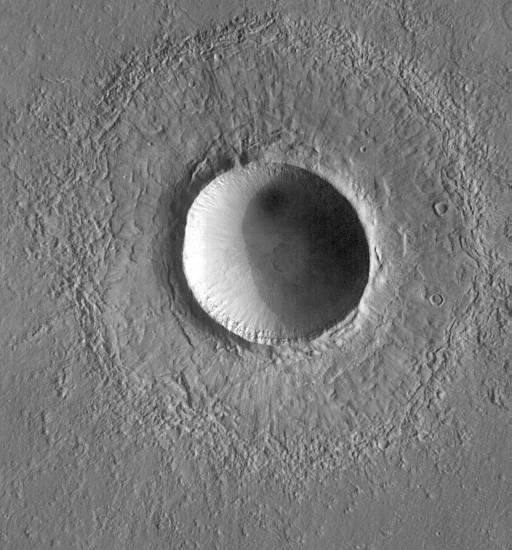
\includegraphics[height=4cm,keepaspectratio]{images/Gre13/Gre13_01.jpg}
		\captionsetup{format=plain}
		\subcaption{Beispiel für einen Krater}
		\label{fig:ex_crater}
	\end{subfigure}
	\hfill
	\begin{subfigure}[t]{0.34\textwidth}
		\centering
		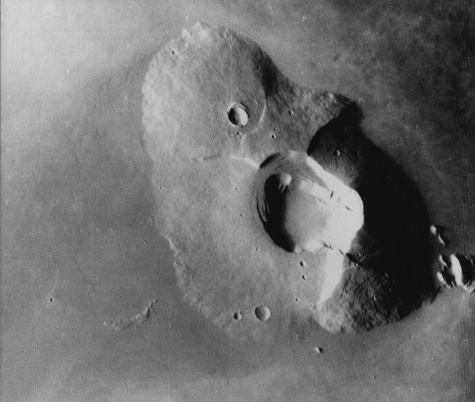
\includegraphics[height=4cm,keepaspectratio]{images/Gre13/Gre13_02.jpg}
		\captionsetup{format=plain}
		\subcaption{Beispiel für einen (ehemaligen) Vulkan}
		\label{fig:ex_vulc1}
	\end{subfigure}
	\hfill
	\begin{subfigure}[t]{0.3\textwidth}
		\centering
		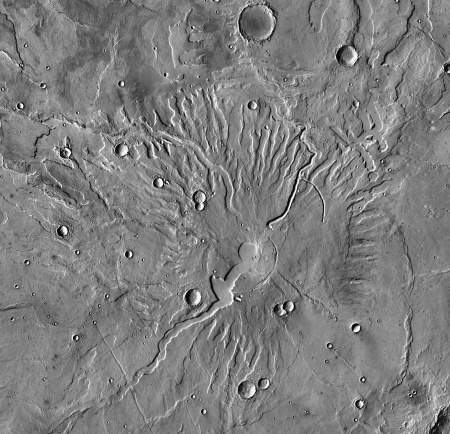
\includegraphics[height=4cm,keepaspectratio]{images/Gre13/Gre13_03.jpg}
		\captionsetup{format=plain}
		\subcaption{Beispiel für einen (ehemaligen) Vulkan mit strahlenförmigen Ausbuchtungen}
		\label{fig:ex_vulc2}
	\end{subfigure}
	\hfill
	\begin{subfigure}[t]{0.35\textwidth}
		\centering
		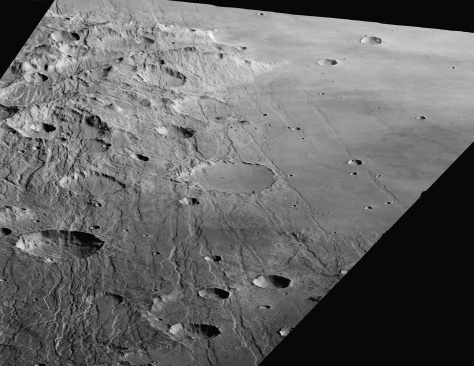
\includegraphics[height=4cm,keepaspectratio]{images/Gre13/Gre13_04.jpg}
		\captionsetup{format=plain}
		\subcaption{Beispiel für mehrere Gräben}
		\label{fig:ex_graben}
	\end{subfigure}
	\hspace{1cm}
	\begin{subfigure}[t]{0.3\textwidth}
		\centering
		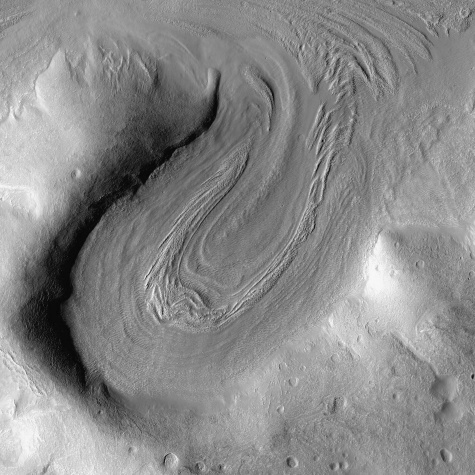
\includegraphics[height=4cm,keepaspectratio]{images/Gre13/Gre13_05.jpg}
		\captionsetup{format=plain}
		\subcaption{Beispiel für einen Gletscher}
		\label{fig:ex_glacier}
	\end{subfigure}
	\hfill
	\caption{Beispiele für Strukturen auf der Marsoberfläche, alle aus \cite[Kap.~7]{greeley_13}}
\end{figure}

\paragraph{}
Diese Faktoren sorgen für eine große Varietät an optisch unterschiedlichen Oberflächen des Mars. Erkennbar sind sie auf Fotografien nur durch das flach einfallende Licht, welches Erhebungen und Täler durch Schatten und hellere Regionen sichtbar macht. Durch diesen Effekt werden auch die unterschiedlichen, zu analysierenden Texturen erkennbar.

\subsection{Remote Sensing Instruments}
\label{ssec:mars_images}

Von der Marsoberfläche existieren verschiedenste Arten von Aufnahmen für unterschiedliche Analysen. Dabei sind gewisse Parameter, wie \zB die aufgenommene Wellenlänge, den Winkel zur Oberfläche, die Auflösung, Brennweite, Ort der Aufnahme und viele weitere wichtig, damit ein Bild zur Analyse einer gewissen Eigenschaft geeignet ist.

Für die hier genutzten Anwendungsfälle eignen sich Instrumente gut, die sichtbares Licht aufnehmen. Obwohl Farbaufnahmen in vielerlei Hinsicht von Vorteil zur Analyse wären, sind diese nicht großflächig vorhanden, daher werden Graustufenaufnahmen als Kompromiss benutzt. Diese besitzen den Vorteil, dass nur ein drittel des Speichers bei den Berechnungen benötigt wird, da statt separaten Rot-, Grün- und Blauwerten nur ein Helligkeitswert gespeichert und verarbeitet werden muss.

Des Weiteren sollten die Bilder eine vergleichsweise hohe Auflösung haben, damit auch kleinere Merkmale gut erkannt werden können. Dies stellt einen Konflikt mit einer weiteren Anforderung dar, da ein Datensatz gesucht wird, der einen Großteil der Oberfläche abdeckt.

Außerdem eignen sich Aufnahmen gut, die senkrecht zur Oberfläche entstanden sind, so dass Objekte auf dieser möglichst denselben Maßstab besitzen.

Unter Berücksichtigung dieser Faktoren ergeben sich \ua zwei geeignete Instrumente:
Die \textit{Context Camera (CTX)} des \textit{Mars Reconnaissance Orbiters} der NASA \cite{malin_07} und die \textit{High Resolution Stereo Camera (HRSC)} des \textit{Mars Express Orbiters} der ESA \cite{hrsc}. Für die eigentlichen Analysen werden Aufnahmen der CTX genutzt, da sie einen Großteil der Oberfläche abdecken, während die panchromatischen Bilder der HRSC zur Evaluierung genutzt wurden, da mit ihnen schon mehrere andere Algorithmen getestet wurden.

\section{Convolutional Neural Networks}
\label{sec:cnn}

Neuronale Netze werden oftmals als eine Weiterentwicklung oder Optimierung des maschinellen Lernens betrachtet: Man setzt auf mehrere Schichten, auch Layers genannt, von vergleichsweise einfachen linearen Funktionen um zur gewünschten Approximation zu kommen. \cite{hardesty_17}

Eine der einfachsten Formen eines neuronalen Netzes besteht aus dem Multilayer-Perceptron: Dieses besteht aus mehreren der zuvor erwähnten Layers, von denen jede mehrere einzelne Perceptronen enthält. Zwischen einer Eingabe- und einer Ausgabe-Schicht existieren somit auch noch eine beliebige Anzahl an sogenannten Hidden Layers.

In diesem Kontext wird ein Perceptron auch als Neuron bezeichnet. Ein typisches Neuron verarbeitet einen Eingabevektor indem es dies mit einem Gewichtungsvektor elementweise multipliziert und anschließend einen Bias-Vektor aufaddiert. Die Addition dieses Bias ist nötig um die gesamte Aktivierungsfunktion entlang der x-Achse verschieben zu können, da sonst manche gewünschten Ergebnisse nicht erreicht werden können. \cite{bias} Ein typisches Neuron ist in \figurename~\ref{fig:neuron} dargestellt. Nach dessen Durchlaufen werden die Elemente dieses Vektor aufaddiert, und auf diese Summe eine Aktivierungsfunktion (\vgl Unterabschnitt~\ref{ssec:activation_layer}) angewandt. Während das Netzwerk trainiert wird, passen die einzelnen Perceptronen diese zwei Vektoren, also die Gewichtungen und die Bias, so an, dass die Ergebnisse weitgehend optimiert werden (\vgl Unterabschnitte\ref{ssec:gradient_descent} und \ref{ssec:backpropagation}). Diese Gewichtungen sind anfangs zufällig bestimmt. \cite{hardesty_17, cs231n} 

\begin{figure}[h!]
	\centering
	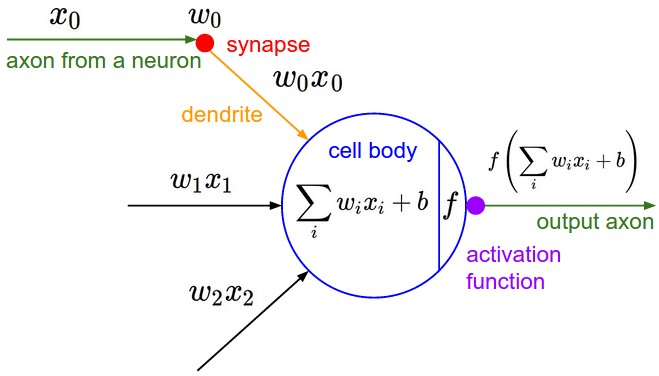
\includegraphics[width=0.5\textwidth,keepaspectratio]{images/LJY19/neuron.jpg}
	\caption{Funktionsweise eines Neurons, aus \cite{cs231n}}
	\label{fig:neuron}
\end{figure}

Die Aneinanderkettung dieser Schichten führt dazu, dass zwischen ihnen eine immer abstraktere Form der Eingabedaten entsteht.

Convolutional Neural Networks beschreiben eine Teilmenge der neuronalen Netze, in der die jeweilige Netzwerkarchitektur mindestens eine Convolutional Layer (auch Faltungsschicht genannt, \vgl Unterabschnitt~\ref{ssec:convolution}) enthält. Die Nutzung dieser Convolutional Layer zieht oft die Nutzung einer Pooling Layer (Unterabschnitt~\ref{ssec:pooling_layer}) mit sich. \cite{deeplearning_16}

Obwohl Convolutional Neural Networks theoretisch dazu geeignet sind die meisten Daten mit einer gitterähnlichen Struktur zu verarbeiten, erfreuen sie sich im Bereich der Bilddatenanalyse der größten Beliebtheit. \cite[Kap.~9]{deeplearning_16} Eine wichtige Ursache für diese Beliebtheit liegt \bspw in dem Erfolg bei dem Bild-Klassifizierungs-Wettbewerb ImageNet. Während dort im Jahr 2011 die Gewinnergruppe mit klassischen Klassifizierungsalgorithmen einen Top-5-Score von $74,3\%$ erzielt hat, wurden im Jahr 2012 mit einem CNN (AlexNet, \cite{alexnet}) erstmals ein Wert von $83,6\%$ erreicht. Von diesem Punkt an wurde die Bestenliste der darauffolgenden Jahre durch Convolutional Neural Networks dominiert. \cite[Kap.~1]{deeplearning_18}

Neben der genannten Objekterkennung eigenen sie sich auch zur Bildsegmentierung. So werden sie \bspw erfolgreich in der Entwicklung von selbstfahrenden Autos eingesetzt. \cite{kaymak_19}

Die Architektur eines typischen, einfachen Convolutional Neural Networks ist wie folgt \cite{cs231n}:

\begin{multline*}
\mathrm{INPUT}\rightarrow\mathrm{CONVOLUTIONAL}\rightarrow\mathrm{ACTIVATION}\\\rightarrow\mathrm{POOLING}\rightarrow\mathrm{FULLYCONNECTED}
\end{multline*}

Da CNNs primär auf Bilddateien angewandt werden, wird von diesem Punkt an von einer Bilddatei als Eingabe ($\mathrm{INPUT}$) ausgegangen. Hier beschreiben die ersten beiden Dimensionen die Breite und Höhe, während die dritte Dimension die Farbwerte für den jeweiligen Pixel angibt. Die Konvolutions-, Aktivierungs-, Pooling- und Fully-Connected-Layers werden in den folgenden Unterabschnitten erläutert.

\subsection{Konvolution}
\label{ssec:convolution}

Die Konvolution, auch Faltung genannt, ist eine mathematische Operation auf zwei beliebigen Funktionen $f(x)$ und $g(y)$, die eine dritte Funktion, die Konvolution $s(x) = f(x)*g(y)$ ergibt, welche beschreibt, wie sich die Verläufe der beiden Funktionen beeinflussen:

\begin{equation}
s(x) = (f*g)(x) = \int_{-\infty}^{\infty} f(y)g(x-y)dy
\end{equation}

In einem Großteil der Anwendungsfälle der Faltung bestehen diese beiden Funktionen aus einer Eingabefunktion $x$ und einem Gewichtungsfunktion $w$, die Ausgabe ist die Merkmalsdimension. In einer praktischen Anwendung wären dies \bspw eine Reihe von zeitabhängigen Messwerten $x(t)$ und eine Gewichtungsfunktion $w(a)$ in Abhängigkeit des Alters der Messung. $w(a)$ wird im Kontext der Konvolution auch Kernel genannt. Für ungültige Zeiten (\bspw Messwerte welche sich in der Zukunft befinden würden) gilt $w=0$ \cite[Kap.~9]{deeplearning_16}:

\begin{equation}
s(t) = (x*w)(t) = \int_{-\infty}^{\infty} x(a)w(t-a)da
\end{equation}

Unter der Annahme, dass die Eingabewerte nicht stetig sondern diskret sind (\bspw zeitliche Messwerte in regelmäßigen Abständen) ergibt sich vereinfacht \cite[Kap.~9]{deeplearning_16}:

\begin{equation}
s(t) = (x*w)(t) = \sum_{a=-\infty}^{\infty}x(a)w(t-a)
\end{equation}

Diese Funktion lässt sich für zweidimensionale Eingabedaten, wie \zB eine Bilddatei $I$ und einen zweidimensionalen Kernel $K$ erweitern \cite[Kap.~9]{deeplearning_16}:

\begin{equation}
S(i,j) = (I*K)(i,j) = \sum_{m}\sum_{n}I(m,n)K(i-m,j-n)
\end{equation}

Eine alternative Betrachtungsweise dieser Formel basiert auf dem Hadamard-Produkt. Angenommen, es existieren eine Matrix $I\in\mathbb{R}^{2}$ und eine Matrix $K\in\mathbb{R}^{m\times n}$.

Sei Matrix $H = K\odot I'$ definiert als Hadamard-Produkt aus $K$ und $I'=I_{x, y}$ mit $x\in[i-m,i]$ und $y\in[j-n,j]$.\\
Dann gilt: $S(i,j)=(I*K)(i,j) = \sum_{m}\sum_{n}I(m,n)K(i-m,j-n)=\sum_{h\in H}h$

Diese Formel ist allerdings nur für Eingabebilder mit nur einem Farbwert pro Pixel gültig, also Graustufenbilder. Für ein Bild mit beliebig vielen Farbwertsdimensionen gilt:

\begin{equation}
S(i,j) = (I*K)(i,j) = \sum_{m}\sum_{n}\sum_{o}I(m,n,o)K(i-m,j-n,o)
\end{equation}

Es ist zu beachten, dass der Farbvektor immer komplett verarbeitet wird, und nicht nur ein Teilausschnitt wie es mit Höhe und Breite geschieht.

\subsection{Convolutional Layer}
\label{ssec:convolutional_layer}

Klassische Schichten von neuronalen Netzen nutzen Matrixmultiplikationen der kompletten Eingabe mit einer Parametermatrix um ihre Ausgaben zu berechnen, \dahe jeder einzelne Ausgabewert entsteht aus einer Berechnung basierend auf jedem einzelnen Eingabewert. Obwohl diese Taktik in vielen Einsatzbereichen gut funktioniert, stößt sie insbesondere bei der Bilddatenanalyse an ihre Grenzen, da sie nicht gut skaliert. \cite{cs231n} So benötigt eine Convolutional Layer zum Erkennen eines Merkmals nur einen Kernel mit einer Anzahl von meistens unter $\SI{100}{\pixel}$. \cite{deeplearning_16} Ein weiterer Pluspunkt besteht daraus, dass durch Convolutional Layers bestimmte Merkmale von unterschiedlichen Stellen der Eingabe extrahiert werden können, wie später beschrieben.

\begin{figure}[H]
	\centering
	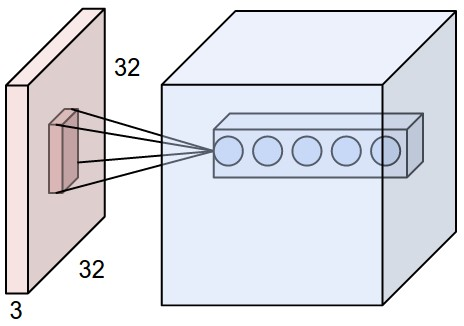
\includegraphics[width=0.4\textwidth,keepaspectratio]{images/LJY19/convolutional.jpg}
	\caption{Funktionsweise der Konvolutions-Schicht, aus \cite{cs231n}}
	\label{fig:convolutional}
\end{figure}

Eine konvolutionelle Schicht besteht aus einer Menge von Neuronen, welche die Eingabe über den eben beschriebenen Konvolutionsoperator $S(i,j)$ auf genau ein Merkmal untersuchen. Daraus folgt, dass die Anzahl der Neuronen in eben dieser Schicht gleich der Größe der entstehenden Merkmalsdimension ist (\vgl \figurename~\ref{fig:convolutional}).

Das Hinzufügen von konvolutionellen Schichten führt allerdings zu mehr Hyperparametern, die optimiert werden können \cite{cs231n}:
\begin{itemize}
	\item Die Dimensionen des Kernels $k_1$ und $k_2$ (obwohl dieser fast immer quadratisch ist, oftmals $3$, $5$ oder $7$)
	\item Die Anzahl der Neuronen/der Merkmalsdimensionen
	\item Die Größe der Schrittweite (auch Stride genannt). Hier wird von einem Wert von $1$ ausgegangen, was die Größe der Ausgabe nicht verändert.
	\item Das Padding, also wie sich die Konvolution an den Rändern der Eingabedaten verhält. Hier wird von Zero-Padding ausgegangen, \dahe dass außerhalb der Ränder der Eingabe alle Werte gleich Null sind. Dies hat ebenfalls zur Folge, dass es die Größe der Ausgabe unverändert lässt.
\end{itemize}

Es gilt es zu beachten, dass der Konvolutionsoperator für alle Werte $i$ und $j$ der Eingabedimensionen aufgerufen wird, so dass die Höhe und Breite der Ausgabe (bis auf einige Ausnahmen) identisch zu denen der Eingabe ist.
Des Weiteren ist der Kernel pro Neuron konstant. Dies hat \ua zur Folge, dass das gleiche Merkmal an verschiedenen Stelle in der Eingabe erkennen kann.

Erhält eine konvolutionelle Schicht mit 12 Neuronen also \bspw ein RGB-Eingabebild der Größe $\SI{64}{\pixel}\times\SI{64}{\pixel}$, so erzeugt es mit einem Stride von $1$ als Ausgabe eine dreidimensionale Matrix der Größe $64\times64\times12$, jede der Schichten der dritten Dimensionen deutet auf das Vorhandensein eines speziellen Merkmals an einer gewissen Stelle im Eingabebild hin.

\subsection{Activation Layer}
\label{ssec:activation_layer}

Auf eine konvolutionelle Schicht folgt fast immer eine Aktivierungsschicht. Diese werden dazu genutzt um eine gewisse Nicht-Linearität in den Verlauf des neuronalen Netzes einzuführen. Nicht-Linearität ist in vielen neuronalen Netzen notwendig, da die Probleme, die sie lösen sollen, nicht-linear sind. \cite[Kap.~6]{deeplearning_16}

Selbst wenn nach der letzten Schicht eines mehrschichtigen neuronalen Netzes eine Aktivierungsschicht hinzugefügt werden würde, hätte dies zur Folge, dass die vorherigen Schichten wie eine einzige lineare Schicht agieren, was keine Vorteile gegenüber einer einzigen Schicht hat. Somit sollte auf jede einzelne Schicht eine Aktivierungsschicht folgen, um verschiedenste, komplizierte Zusammenhänge zwischen Ein- und Ausgabedaten besser approximieren zu können. \cite[Kap.~3]{deeplearning_18}

In \figurename~\ref{fig:activations} sind drei der am meisten Verbreiteten Aktivierungsfunktionen zu sehen.

\begin{figure}[h!]
	\begin{subfigure}{0.33\textwidth}
		\centering
		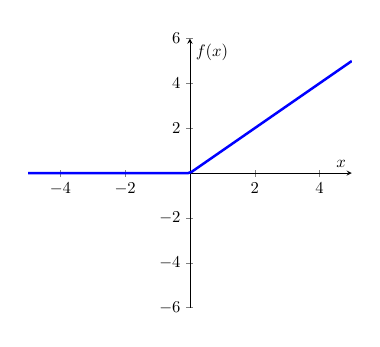
\begin{tikzpicture}[scale=0.6]
			\begin{axis}[
				axis lines = middle,
				xlabel = {$x$},
				ylabel = {$f(x)$},
				domain=-5:5,
				]
				\addplot[draw=blue,samples=100,domain=-5:5,line width=1.5]{max(0,x)};
				\addplot[draw opacity=0,domain=-5:5]{1.2*x};
			\end{axis}
		\end{tikzpicture}
		\subcaption{ReLU:\\$f(x)=\mathrm{max}\{0,x\}$}
		\label{fig:relu}
	\end{subfigure}
	\begin{subfigure}{0.32\textwidth}
		\centering
		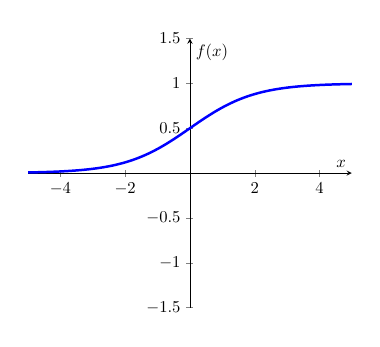
\begin{tikzpicture}[scale=0.6]
			\begin{axis}[
				axis lines = middle,
				xlabel = {$x$},
				ylabel = {$f(x)$},
				domain=-5:5,
				]
				\addplot[draw=blue,samples=100,domain=-5:5,line width=1.5]{1/(1+e^(-x))};
				\addplot[draw opacity=0,domain=-5:5]{0.3*x};
			\end{axis}
		\end{tikzpicture}
		\subcaption{Sigmoid:\\$f(x)={1}/{(1+e^{-x})}$}
		\label{fig:sigmoid}
	\end{subfigure}
	\begin{subfigure}{0.33\textwidth}
		\centering
		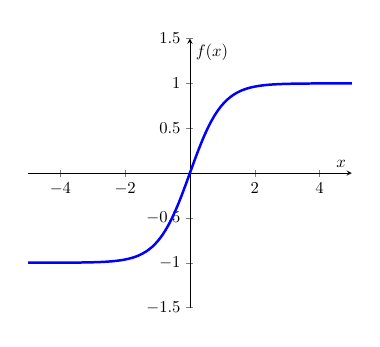
\begin{tikzpicture}[scale=0.6]
			\begin{axis}[
				axis lines = middle,
				xlabel = {$x$},
				ylabel = {$f(x)$},
				domain=-5:5,
				]
				\addplot[draw=blue,samples=100,domain=-5:5,line width=1.5]{tanh(x)};
				\addplot[draw opacity=0,domain=-5:5]{0.3*x};
			\end{axis}
		\end{tikzpicture}
		\subcaption{tanh:\\$f(x)=tanh(x)$}
		\label{fig:tanh}
	\end{subfigure}
	\caption{Drei Aktivierungsfunktionen}
	\label{fig:activations}
\end{figure}

Die intuitivste Aktivierungsfunktion, die Einheitssprungfunktion, wird in neuronalen Netzen nur für Binärklassifizierungsprobleme in der letzten Schicht genutzt. Dies rührt daher, dass sie keine Ableitung besitzt und daher nicht zum Lernen über Backpropagation (\vgl Unterabschnitt~\ref{ssec:backpropagation}) geeignet ist.

Die ReLU-Aktivierungsfunktion (\vgl \figurename~\ref{fig:relu}) ist die wohl einfachste (nicht-lineare) Funktion, die als Aktivierungsfunktion geeignet ist. Diese Einfachheit führt zu einer vergleichsweise guten Performance, und deshalb großer Beliebtheit in neuronalen Netzen mit vielen Schichten. Ihr Nachteil besteht darin, dass für Bereich $x<0$, praktisch gesehen kein Lernprozess stattfindet, da sie dort immer $0$ beträgt. \cite{kizrak_19} Zur Lösung dieses Problemes wurden Alternativen, wie \zB die Leaky-ReLU-Funktion entwickelt.

Die Sigmoid-Funktion eignet sich gut als Aktivierungsfunktion, da sie im Bereich nahe der y-Achse eine hohe Steigung aufweist, während die Veränderungen in anderen Bereichen relativ klein ausfallen. Damit eignet sie sich insbesondere gut zur Klassifizierung. \cite{kizrak_19}

Die $tanh(x)$-Funktion ist in ihrer Rolle als Aktivierungsfunktion relativ ähnlich zur Sigmoid-Funktion, mit dem Unterschied dass sie im negativen x-Bereich auch ins Negative geht, statt sich an $0$ anzunähern. Wie die Sigmoid-Funktion eignet sie sich gut zur Klassifizierung, je nach Anwendungsfall sogar besser, da ihre Ableitung nahe der y-Achse steiler ist. \cite{kizrak_19}

Es existieren noch weitere Aktivierungsfunktionen, diese zu Analysieren ist allerdings außerhalb des Rahmens dieser Arbeit.

\subsection{Pooling Layer}
\label{ssec:pooling_layer}

Konvolutionelle Schichten in neuronalen Netzen können die selben Merkmale von unterschiedlichen Stellen extrahieren. Die Position, an der diese Merkmale erkannt wurden, werden auch an die nächste Schicht weitergegeben, \dahe kleine Veränderungen an der Position eines Merkmals führen zu einer veränderten Merkmalsdimension. \cite{brownlee_19} Dies kann insbesondere beim Einsatz von mehreren konsekutiven Convolutional Layers zu einer erhöhten Störanfälligkeit führen, deshalb wird oftmals eine Pooling-Layer dazu eingesetzt, das resultierende Netzwerk invariant zu einzelnen Merkmalspositionen zu machen. Des Weiteren dient eine Pooling-Layer dazu, Informationen aus verschiedenen Bildbereichen zu abstrahieren und langsam global zu aggregieren. \cite{deeplearning_16}

\begin{figure}[h!]
	\centering
	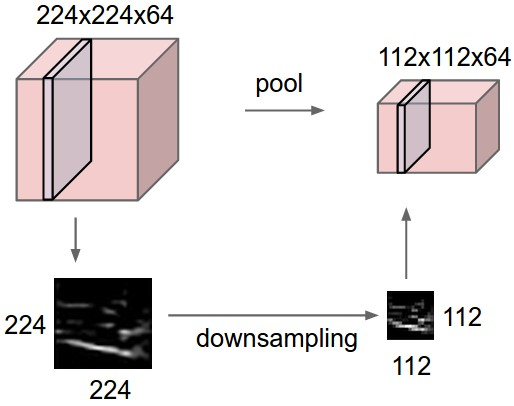
\includegraphics[width=0.37\textwidth,keepaspectratio]{images/LJY19/pool.jpg}
	\caption{Funktionsweise der Pooling-Layer, aus \cite{cs231n}}
	\label{fig:pooling}
\end{figure}

Ein weiteres Problem des Einsatzes von ausschließlich konvolutionellen Schichten besteht daraus, dass sie schnell zu einem hohen Anstieg der Parameterzahl im Netzwerk führen können: Jede neue Schicht erzeugt einen weiteren Datenwürfel der Größe $H\times W\times F$, wobei $H$ und $W$ die Höhe und Breite des Eingabebildes, und $F$ die Größe der Merkmalsdimension ist. Alle diese Werte werden im Training des neuronalen Netzes optimiert, was zu Performanceeinbüßungen führen kann. \cite{cs231n}

Die Pooling-Schicht verarbeitet alle Merkmalsdimensionen ihrer Eingabe unabhängig voneinander.

Für jede Merkmalsdimension überlauft der rezeptive Bereich -- ähnlich zur Konvolutions-Schicht -- die jeweilige Schicht des Würfels in Höhe und Breite, und berechnet je nach Pooling-Art einen Wert, welcher als positionsabhängige Ausgabe weitergeleitet wird. Dieser Prozess ist in \figurename~\ref{fig:pooling} dargestellt.

Dieser Prozess besitzt zwei Hyperparameter: Die Stride (Schrittweite) $S$ und die eigentliche Größe $F_1\times F_2$. \cite{cs231n}

\begin{figure}[H]
	\centering
	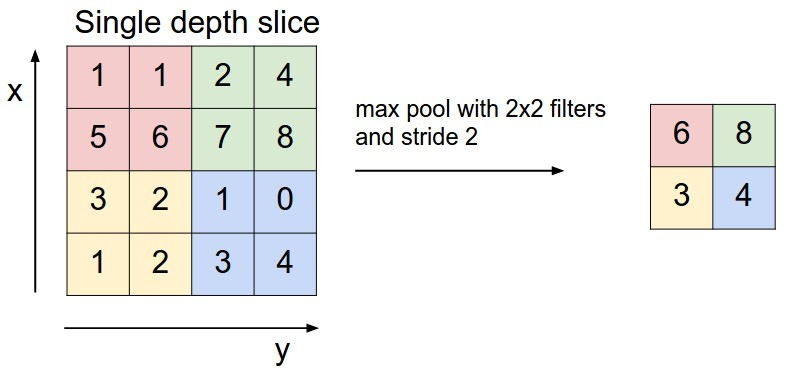
\includegraphics[width=0.6\textwidth,keepaspectratio]{images/LJY19/maxpool.jpg}
	\captionsetup{width=0.6\textwidth}
	\caption{Max-Pooling anhand eines Beispiels, aus \cite{cs231n}}
	\label{fig:maxpooling}
\end{figure}

Beim Max-Pooling übernimmt die Poolingoperation den maximalen Wert des von ihr überdeckten Eingabebereiches (\vgl \figurename~\ref{fig:maxpooling}).

\subsection{Fully Connected Layer}
\label{ssec:fully_connected_layer}
Viele Convolutional Neural Networks besitzen (mindestens) eine Fully Connected Layer. Das Ziel dieser besteht daraus, die Resultate der konvolutionellen und Pooling-Schichten zu klassifizieren, da diese nur die Wahrscheinlichkeiten zurückgeben, mit der ein gewisses Merkmal an einer gewissen Position erkannt wird. Aus diesem Grund werden oft eine oder mehrere Fully Connected Layers am Ende eines ansonsten fertigen neuronalen Netzes eingesetzt. \cite{geva}

Die Funktionsweise einer Fully Connected Layer ist identisch zu einer Schicht eines Multilayer-Perceptrons, welches in Abschnitt~\ref{sec:cnn} beschrieben ist.

\subsection{Batch Normalization}
\label{ssec:bn}

Die in \cite{ioffe_15} vorgestellte Technik der Batch Normalization erleichtert die korrekte Initialisierung eines neuronalen Netzes. Das Ziel des genannten Papers bestand ursprünglich daraus, die \enquote{Internal Covariante Shift} zu minimieren, also wie sehr sich die Verteilung der Eingaben der folgenden Schichten verändert, wenn sich die Parameter einer vorherigen Schicht verändern. Sie wird dementsprechend normalerweise zwischen Fully Connected/Convolutional Layers und der darauffolgenden, nichtlinearen Aktivierungsfunktion eingefügt. \cite{cs231n}

Mathematisch betrachtet funktioniert diese Schicht, indem sie die Gauß-Verteilung ihrer Eingabe berechnet, und diese Ergebnisse an die nächste Schicht im Netzwerk weitergibt. \cite{cs231n} Bekommt sie so \bspw aus einer Quelle Eingabewerte im Intervall $\left[0, 1\right]$, und aus einer weiteren Quelle Werte aus $\left[0, 1000\right]$, so werden diese Werte (bei gleicher Gewichtung der Eingabewerte der nächsten Schicht) sehr unterschiedlich gewertet. Dieses Problem wird durch die Batchnormalisierung behoben.

In \cite{santurkar_18} wurde zusätzlich gezeigt, dass durch die Nutzung von Batch Normalization auch die Verlustfunktion geglättet wird, was oft zu einer geringeren Dauer des Training führt. Insgesamt erhöht Batch Normalization also die Stabilität eines Netzes.

\subsection{Loss Function}
\label{ssec:loss_function}

Wie gut ein neuronales Netz eine Zielfunktion approximiert wird über den Loss gemessen, \dahe das Ziel eines neuronalen Netzes besteht daraus, den Loss in jeder Iteration weiter zu minimieren. DIe Lossfunktion, auch Verlustfunktion genannt, beschreibt, wie stark sich die vom Netz berechneten Werte von den zu erzielenden Werten (beim überwachten Lernen meistens die Ground Truth) unterscheiden.

Auch hier existieren verschiedenste Loss-Funktionen. Im Folgenden wird genauer auf den Cross-Entropy-Loss eingegangen. Dieser ist besonders für Klassifizierungsprobleme geeignet. Er ist definiert als \cite{cs231n}:

\begin{equation}
H(p,q) = -\sum_x p(x)\log q(x)
\end{equation}

Dabei gibt $p$ die korrekten Klassen als one-hot-kodierter Vektor an: $p$ ist also ein Vektor mit $n$ Elementen, wobei $n$ die Anzahl der möglichen Klassen ist. 

Es gilt: $f_i$ ist gleich dem $i$-ten Element eines Eingabevektors $f$.

Eine korrekte Klasse wird mit einer $1$ am entsprechenden Element im Vektor kodiert, alle anderen Felder sind gleich $0$. Ist für die jeweilige Eingabe nun \bspw die $m$-te Klasse korrekt, so gilt $p_m=1$ und $p_{\left[1,m-1\right]} = p_{\left[m+1,n\right]} = 0$. Es ist zu beachten, dass der Cross-Entropy-Loss ausschließlich die Wahrscheinlichkeiten für korrekte Klassen bewertet.

$q$ hingegen gibt die berechnete Wahrscheinlichkeit an, dass eine jeweilige Klasse auf die Eingabe zutrifft. Da für $q$ eine Wahrscheinlichkeitsverteilung, welche sich auf $1$ aufsummiert benötigt wird, wird als dessen Eingabe meistens die Softmax-Funktion der vorhergehenden Werte genutzt. Die Softmax-Funktion kann wie die ReLU- oder die Sigmoid-Funktion als Aktivierungsfunktion betrachtet werden. Sie ist definiert durch \cite{cs231n}:

\begin{equation}
S_i=\frac{e^{f_i}}{\sum_j e^{f_j}}
\end{equation}

Kombiniert ergibt sich so also für den Cross-Entropy-Loss \cite{cs231n}:

\begin{equation}
L_i = -\sum_x p(x)\log\left(\frac{e^{f_{y_i}}}{\sum_j e^{f_i}}\right)
\end{equation}

Da für alle außer eine Klasse gilt $p=0$, lässt sich die Summe entfernen:

\begin{equation}
L_i = -\log\left(\frac{e^{f_{y_i}}}{\sum_j e^{f_i}}\right)
\end{equation}


Für den durchschnittlichen Loss über alle Klassifizierungen ergibt sich so:

\begin{equation}
L = \frac{1}{N}\sum_{i=1}^{N}L_i
\end{equation}

Hier ist allerdings zu beachten, dass es für ein neuronale Netz mehrere optimale Gewichtungen und Bias geben kann: Würde man \bspw alle Gewichtungen mit dem selben Skalar multiplizieren, würden diese immer noch zu dem selben Ergebnis führen. Um möglichst kleine Gewichtungen und Biase zu bestimmen, wird ein Regularisierungsterm eingeführt um die Gewichtungen möglichst gering zu halten \cite{cs231n}:

\begin{equation}
\label{eqn:def_loss}
L = \frac{1}{N}\sum_{i=1}^{N}L_i + \lambda R(W)
\end{equation}

mit $\lambda$ als einem Hyperparameter zur Gewichtung und

\begin{equation}
R(W) = \sum_k\sum_l W^2_{k,l}
\end{equation}

\subsection{Gradientenverfahren}
\label{ssec:gradient_descent}

Das Ziel eines neuronalen Netzes besteht daraus, die Werte der Lossfunktionen weitgehend zu minimieren. Dies wäre rein theoretisch durch klassische Analysis möglich, indem man die Ableitungen der Funktionen Netzes berechnet und aus diesen anschließend die Extrempunkte. In der Praxis allerdings, besitzt so ein Netzwerk viel zu viele Variablen, als dass die Extremalstellen in einem Annehmbaren Zeitraum berechnet werden könnten. \cite[Kap.~1]{nielsen_15} AlexNet, der Gewinner der ImageNet-Challenge 2012 besitzt \bspw etwa 60 Millionen trainierbare Parameter. (\Vgl Abschnitt~\ref{sec:cnn})

Die Funktion $C(w, b)$ sei die zu minimierende Lossfunktion in Abhängigkeit von den Gewichtungen und Bias des neuronalen Netzes. Zur einfacheren Erklärung gilt, \oBdA, dass im Netzwerk nur zwei trainierbare Parameter existieren. Somit ist das Ziel, die Parameter der Funktion $C(v_1, v_2)$ so zu optimieren, dass das Funktionsergebnis minimiert wird. Grafisch ist eine Beispielfunktion $C$ in \figurename~\ref{fig:valley} dargestellt.

\begin{figure}[h!]
	\centering
	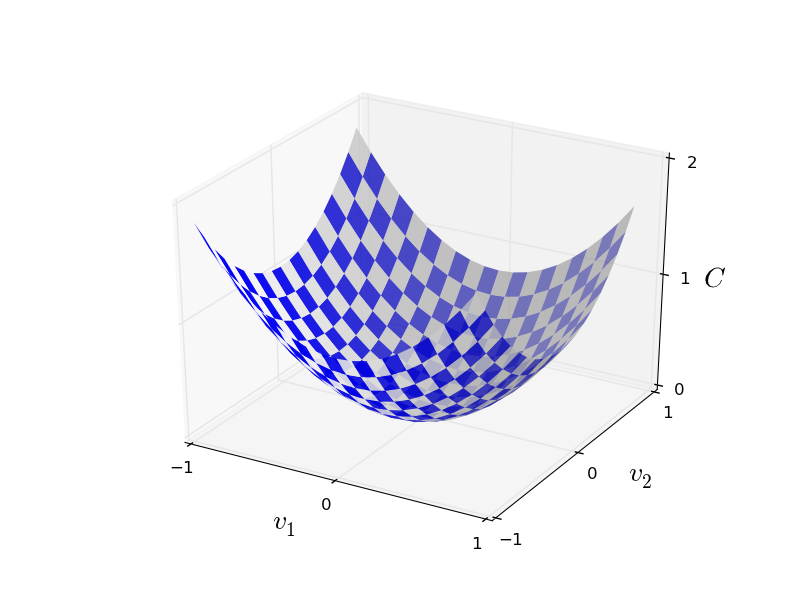
\includegraphics[width=0.45\textwidth,keepaspectratio]{images/Nie15/Nie15_01.png}
	\caption{Funktion $C$ in Abhängigkeit von $v_1$ und $v_2$, aus \cite[Kap.~1]{nielsen_15}}
	\label{fig:valley}
\end{figure}

Das Gradientenverfahren beschreibt einen Prozess zur Lösung dieses Problems: Bei diesem Verfahren beginnt man bei einem Startpunkt auf dem Funktionsgraphen. Von dort aus wird ermittelt, in welche Richtung der Graph (hier) absteigend verläuft. Man schreitet nun in diese Richtung und wiederholt das Verfahren. Dies geschieht so lange, bis man an einem Punkt angelangt, von welchem aus es in keine Richtung mehr bergab geht. Dieser Punkt ist ein lokales Minimum. Es gilt zu beachten, dass die Weite des jeweiligen Schrittes variabel ist: Es kann somit geschehen, dass am Ende des Verfahrens, der jeweilige Punkt um das lokale Minimum herum schwankt.

Der Prozess lässt sich anschaulich dadurch darstellen, dass man einen Ball an einem beliebigen Punkt auf dem Graphen fallen lässt. Ignoriert man Reibung, Trägheit und andere physikalische Eigenschaften, rollt dieser immer in Richtung des nächsten lokalen Minimums.

Mathematisch betrachtet ändert sich von einem beliebigen Punkt aus der Wert der Funktion $C$ um $\Delta C$, wenn jeweils eine Entfernung von $\Delta v_1$ in $v_1$-richtung, und $\Delta v_2$ in $v_2$-richtung zurückgelegt wird: \cite[Kap.~1]{nielsen_15}

\begin{equation}
\label{eqn:def_deltaC}
\Delta C\approx \frac{\partial C}{\partial v_1}\Delta v_1 + \frac{\partial C}{\partial v_2}\Delta v_2
\end{equation}

Diese Gleichung ist nur eine Annäherung, da statt der Steigung zwischen $v_1$ und $\Delta v_1$ nur die Steigung an der Stelle $v_1$ betrachtet wird. Dies gilt analog für $v_2$.
Es gelte nun: $\Delta v$ sei der Vektor der Differenzen in $v$

\begin{equation}
\Delta v\equiv (\Delta v_1, \Delta v_2)^T
\end{equation}

Und $\nabla C$ sei der Gradient von $C$:

\begin{equation}
\nabla C\equiv \left(\frac{\partial C}{\partial v_1}, \frac{\partial C}{\partial v_2}\right)^T
\end{equation}

Durch Einsetzen in Gleichung~\ref{eqn:def_deltaC} gilt nun:

\begin{equation}
\Delta C \approx \nabla C\Delta v
\end{equation}

Es sei nun:

\begin{equation}
\label{eqn:let_deltav}
\Delta v = -\eta\nabla C
\end{equation}

wobei $\eta$ ein beliebiger, positiver Wert sei. Dieser wird auch \textit{learning rate} --~Lernrate~-- genannt. $\eta$ sollte so klein gewählt werden, als dass Gleichung~\ref{eqn:def_deltaC} eine gute Annäherung bleibt \cite[Kap.~1]{nielsen_15}, aber groß genug, als dass die Anzahl der nötigen Iterationen gering gehalten wird. Daraus folgt:

\begin{equation}
\Delta C\approx -\eta\nabla C\cdot\nabla C= -\eta\left|\left|\nabla C\right| \right|^2
\end{equation}

Da $\left|\left|\nabla C\right| \right|^2$ immer größer/gleich 0 ist, verringert sich der Wert $C$ solange die Annahme in Gleichung~\ref{eqn:let_deltav} gilt. 

Es werden also $\Delta v_1$ und $\Delta v_2$ nun in jeder Iteration nach dieser Annahme gewählt, um den Wert von $C$ in jedem Durchlauf des Prozesses weiter zu verringern. Nach ausreichend vielen Iterationen erhält man die Koordinaten eines lokalen Minimums.

Der Prozess des Gradientenverfahrens stößt allerdings in diesem Anwendungsfall an seine Grenzen, da hier globale statt lokale Extrempunkte gesucht werden. Ein weiteres Problem besteht daraus, dass die Verlustfunktion $C$ vergleichsweise komplex ist, da sie aus dem Durchschnitt der Verlustfunktionen aller Klassen besteht (\vgl Gleichung~\ref{eqn:def_loss}).

Beide Probleme lassen sich durch die Nutzung des stochastischen Gradientenverfahrens lösen: Dabei wird, pro Iteration, statt der Durchschnitt aller Lossfunktionen, nur eine einzigen, zufällig ausgewählten Verlustfunktion betrachtet. \cite{kathuria_18}

Sollte man nun an einem lokalen Minimum einer Verlustfunktion angelangt sein, so wird in der nächsten Iteration eine andere Funktion betrachtet, welche an dieser Stelle möglicherweise kein Minimum besitzt.

Des Weiteren wird der Rechenaufwand drastisch reduziert, da die Startkoordinaten des jeweils nächsten Durchlaufs anhand nur einer Funktion, statt anhand des Durchschnitts aller Verlustfunktionen berechnet wird.

Ein praktischer Nachteil des stochastischen Gradientenverfahrens besteht allerdings daraus, dass bei dem klassischen Gradientenverfahren die Ergebnisse der unterschiedlichen Verlustfunktionen parallel berechnet werden können, dies beim stochastischen Gradientenverfahren nicht möglich ist, da das Ergebnis einer Iteration auf dem der vorherigen Iteration basiert. Es wird also ein Kompromiss beschlossen, in dem in jedem Durchgang eine Teilmenge der Verlustfunktionen genutzt wird. \cite{kathuria_18} Dies vereint die Vorteile beider Gradientenverfahren (die Meidung der lokalen Minima des stochastischen Gradientenverfahrens und den möglichen Parallellismus des klassischen Gradientenverfahrens).

Alle in diesem Unterabschnitt erklärten Verfahren lassen sich analog auf eine größere Anzahl an Parametern anwenden.

\subsection{Backpropagation}
\label{ssec:backpropagation}

Um das Gradientenverfahren anwenden zu können, wird der Gradient $\nabla C_x$ der Verlustfunktion $C_x$ benötigt. Da in einem neuronalen Netz der Trainingsdatensatz fest steht, muss dieser Gradient nur in Abhängigkeit der Gewichtungen $w$ und Biase $b$ des Netzes gebildet werden. Gesucht werden also $\frac{\partial C}{\partial w}$ und $\frac{\partial C}{\partial b}$ für jeweils jede Gewichtung und Bias des Netzes.

Außerdem sei die Aktivierung, also die Ausgabe eines beliebigen Neurons definiert als: \cite[Kap.~2]{nielsen_15}

\begin{equation}
a_j^l = \sigma\left(\sum_k w_{jk}^l a_k^{l-1}+b_j^l\right)
\end{equation}

Sei nun $w^l$ die Gewichtungsmatrix einer Schicht $l$. Ein Wert $w_{jk}^l$ gibt also wie oben die Gewichtung vom $k$-ten Neurons in der $\left(l-1\right)$-ten Schicht zum $j$-ten Neuron in der $l$-ten Schicht. Analog existiert ein Biasvektor $b^l$, welcher für einen Wert $b_j^l$ den Bias des $j$-ten Neurons der $l$-ten Schicht angibt. $\sigma$ ist die Aktivierungsfunktion des jeweiligen Neurons. Es existeiren insgesamt $L$ Schichten.

Diese Gleichung lässt sich in Vektorform wie folgt darstellen: (nach \cite[Kap.~2]{nielsen_15})

\begin{equation}
a^l = \sigma\left(w^l a^{l-1}+b^l\right)
\end{equation}

Ein wichtiger Vorteil dieser vektorisierten Formeln ist (neben ihrer Lesbarkeit) die Möglichkeit, sie parallel einfacher zu berechnen.

Des Weiteren seien die gewichteten Eingaben $z^l$ einer Schicht $l$ definiert durch: (nach \cite[Kap.~2]{nielsen_15})

\begin{equation}
z^l \equiv w^l a^{l-1} + b^l
\end{equation}

Daraus folgt $a^l=\sigma\left(z^l\right)$.

Durch Backpropagation kann immer nur das Fehlersignal $\delta_j^l$ des $j$-ten Neurons der $l$-ten Schicht berechnet werden. Dieser ist definiert als: (nach \cite[Kap.~2]{nielsen_15})

\begin{equation}
\delta_j^l \equiv \frac{\partial C}{\partial z_j^l} = \frac{\partial C}{\partial a_j^l}\frac{\partial a_j^l}{\partial z_j^l} = \frac{\partial C}{\partial a_j^l}\sigma'\left(z_j^l\right)
\end{equation}

Er gibt also das Verhältnis der Veränderung der Verlustfunktion des Netzes zur Veränderung einer gewichtete Eingabe $z_j^l$ an. Für die Ausgabe der letzten Schicht $L$ des Netzwerkes folgt:

\begin{equation}
\delta_j^L = \frac{\partial C}{\partial a_j^L}\sigma'\left(z_j^L\right)
\end{equation}

Dies lässt sich auch in vektorisierter Form schreiben: (nach \cite[Kap.~2]{nielsen_15})

\begin{equation}
\label{eqn:bp1}
\delta^L = \nabla_{a^L} C\odot\sigma'\left(z^L\right)
\end{equation}

Wie in Unterabschnitt~\ref{ssec:convolution} beschreibt der $\odot$-Operator das Hadamard-Produkt der jeweiligen Matrizen und $\nabla_{a^l} C$ ist der Vektor aller partiellen Ableitungen $\frac{\partial C}{\partial a_j^l}$ einer Schicht $l$.

Um den Fehler $\delta^l$  anhand des Fehlers der nächsten Schicht $\delta^{l+1}$ wird Gleichung~\ref{eqn:bp1} so umgeformt, dass sie die Veränderung von $C$ in Abhängigkeit von $z^{l+1}$ statt in Abhängigkeit von $z^{l}$ darstellt. Die vollständige Herleitung ist in \cite[Kap.~2]{kathuria_18} zu finden. Aus ihr ergibt sich:

\begin{equation}
\label{eqn:bp2}
\delta^l =\left(\left(w^{l+1}\right)^T\delta^{l+1}\right)\odot\sigma'\left(z^l\right)
\end{equation}

Durch die Kombination der Gleichungen~\ref{eqn:bp1} und \ref{eqn:bp2} lässt sich der Fehler in einer belibigen Schicht berechnen.

Um nun anhand der Fehler die jeweiligen Gradienten der Verlustfunktion in Bezug auf die Gewichtungen und Biase zu berechnen gilt nun nach der Herleitung in \cite[Kap.~2]{kathuria_18}:

\begin{eqnarray}
\label{eqn:bp3}
\frac{\partial C}{\partial b_j^l} &=& \delta_j^l\\
\label{eqn:bp4}
\frac{\partial C}{\partial w_{jk}^l} &=& a_k^{l+1}\delta_j^l
\end{eqnarray}

Mithilfe dieser Formeln lässt sich nun, wie für das Gradientenverfahren benötigt, effizient der Gradient der Verlustfunktion $C$ für eine Eingabe $x$ in Abhängigkeit bestimmter Parameter berechnen. Es sein $a^1=x$. (nach \cite[Kap.~2]{nielsen_15})

Zuerst werden für jedes Neuron jeder Schicht $l$ die Aktivierung und die gewichtete Eingabe berechnet:
\begin{eqnarray}
z^{l}&=& w^{l}a^{x-1}+b^l\\
a^{l}&=&\sigma\left(z^{l}\right)
\end{eqnarray}

Anschließend wird der Fehlervektor der letzten Schicht $L$ berechnet (\vgl Gleichung~\ref{eqn:bp1}):
\begin{equation}
\delta^{L}=\nabla_{a^L}C_x\odot\sigma'\left(z^{L}\right)
\end{equation}

Dieser wird nun rückwärts durch die Schichten propagiert (\vgl Gleichung~\ref{eqn:bp2}):
\begin{equation}
\delta^{l}=\left(\left(w^{l+1}\right)^T\delta^{l+1}\right)\odot\sigma'\left(z^{l}\right)
\end{equation}

Daraus lassen sich mithilfe der Formeln~\ref{eqn:bp3} und \ref{eqn:bp4} die Gradienten der Verlustfunktion in Bezug auf die Gewichtungen und Biase herleiten:

\begin{eqnarray}
\frac{\partial C}{\partial w_{jk}^l}&=&a_k^{l-1}\delta_j^l\\
\frac{\partial C}{\partial b_{j}^l}&=&\delta_j^l
\end{eqnarray}

Da nun diese Gradienten bekannt sind, lässt sich das in Unterabschnitt~\ref{ssec:gradient_descent} beschriebene Gradientenverfahren erfolgreich anwenden.